\documentclass[italian,10pt,a4paper]{report}
\usepackage[T1]{fontenc}
\usepackage{graphicx}
\usepackage{mathtools}
\usepackage{amssymb}
\usepackage{amsthm}
\usepackage{thmtools}
\usepackage[dvipsnames]{xcolor}
\usepackage{nameref}
\usepackage{longtable}
\usepackage{tabularray}
\usepackage{tabularx}
\usepackage{microtype}
\usepackage{cancel}
\usepackage{babel}
\usepackage{enumitem}
\usepackage[hidelinks]{hyperref}
\usepackage{tcolorbox}
\usepackage{tikz}
\usetikzlibrary{shapes, positioning}
\usepackage{wrapfig, subcaption}
{\renewcommand{\arraystretch}{2}%
\title{Appunti di parallel programming}
\author{Riccardo Torre\and Michele Perlotto}
\newtheoremstyle{note}% <name>
{3pt}% <Space above>
{3pt}% <Space below>
{}% <Body font>
{}% <Indent amount>
{\bfseries}% <Theorem head font>
{:}% <Punctuation after theorem head>
{.5em}% <Space after theorem headi>
{}% <Theorem head spec (can be left empty, meaning `normal')>
\theoremstyle{note}
\newtheorem{exercise}{Esercizio}[section]
\newtheorem{solution}{Soluzione}[section]
%\theoremstyle{definition}
\begin{document}
	\maketitle
	\tableofcontents
	\chapter{Concetti fondamentali}
\section{Introduzione alla programmazione parallela}
Il software senza la parallelizzazione viene eseguito su una singola unità centrale di elaborazione (CPU). Il problema viene suddiviso in una serie discreta di istruzioni che vengono eseguite una dopo l'altra e una per volta come in figura \ref{fig:serial-computation}.

\begin{figure}[th]
	\centering
	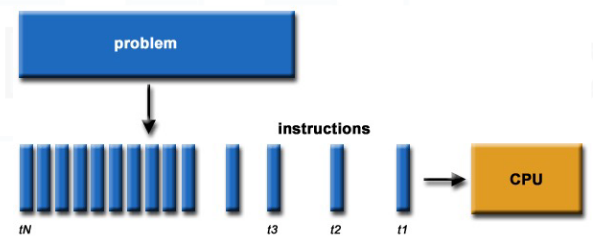
\includegraphics[width=0.8\linewidth]{img/serial-computation}
	\caption{computazione seriale.}
	\label{fig:serial-computation}
\end{figure}

Il \textbf{calcolo parallelo} consiste nell'uso simultaneo di più risorse di calcolo per risolvere un problema computazionale impiegando più CPU per eseguire le operazioni. Un problema viene suddiviso in parti più discrete, ognuna delle quali può essere risolta in modo \textbf{indipendente} e \textbf{contemporaneo}. Successivamente ogni parte è ulteriormente suddivisa in una serie di istruzioni che vengono eseguite simultaneamente su diverse CPU. Questo approccio consente di accelerare notevolmente il processo di calcolo rispetto al calcolo seriale.
\subsubsection*{Motivazioni}
\begin{enumerate}
	\item risparmiare tempo e denaro;
	\item risolvere problemi più grandi;
	\item fornire concorrenza;
	\item utilizzo di risorse non locali.
\end{enumerate}
\subsection*{Un ripasso dell'architettura di Von Neumann}

\begin{wrapfigure}{r}{0.35\linewidth}
	\centering
	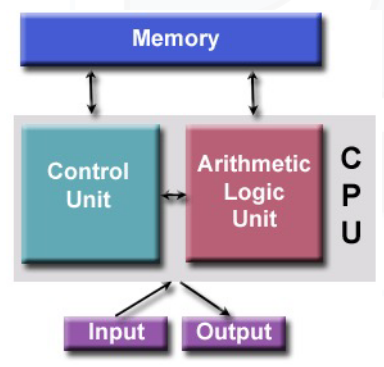
\includegraphics[width=.7\linewidth]{img/von-neumann}
	\caption{architettura di Von Neumann.}
	\label{fig:von-neumann}
\end{wrapfigure} 
Comprende la \textbf{memoria}, l'\textbf{unità di controllo}, l'\textbf{unità aritmetico logica} e le \textbf{periferiche di input/output}. La lettura e la scrittura sulla \textbf{RAM} -- \textbf{\textit{random access memory}} viene utilizzato per memorizzare sia istruzioni che dati del programma. L'\textbf{unità di controllo} recupera le istruzioni e i dati dalla memoria, decodifica le istruzioni e coordina sequenzialmente le operazioni per portare a termine il task\footnote{Generalmente con task ci si riferisce ad un compito.} programmato. L'\textbf{unità aritmetico logica} svolge le operazioni aritmetiche di base. L'\textbf{I/O} è l'interfaccia con cui avviene l'interazione uomo-macchina.

\subsection{Tassonomia classica di Flynn}
La tassonomia classica di Flynn distingue le architetture dei computer multiprocessore in base a come possono essere classificate lungo le due dimensioni indipendenti di \textbf{istruzioni} e \textbf{dati}.
\begin{figure}[th]
	\centering
	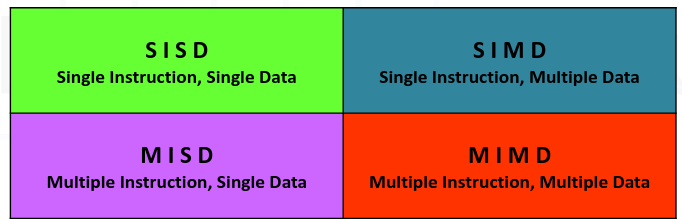
\includegraphics[width=0.7\linewidth]{img/flynn}
	\caption{matrice di flynn.}
	\label{fig:flynn}
\end{figure}

\subsubsection*{Legenda figura \ref{fig:sisd}}
\begin{enumerate}
	\item IS -- \textit{Instruction stream}. Le istruzioni di un programma da eseguire;
	\item DS -- \textit{Data Stream}. Operandi e risultati su cui il programma sta lavorando;
	\item PU -- \textit{Processing Unit}. Unità funzionale composta da ALU e registri. Esegue le istruzioni;
	\item MM -- \textit{Main Memory}. La memoria in cui vengono allocati dati e istruzioni.
\end{enumerate}
\clearpage
\subsection*{SISD -- Single Istruction Single Data}
\begin{figure}[th]
	\centering
	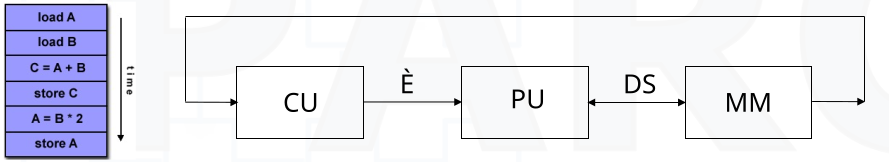
\includegraphics[width=0.7\linewidth]{img/sisd}
	\caption{sisd.}
	\label{fig:sisd}
\end{figure}\noindent
CU esegue le istruzioni dalla MM, mentre PU esegue le istruzioni interagendo con la MM per modificare i dati. È un'architettura standard di Von Neumann, in cui ciascun programma esegue e si affida ad un flusso di dati singolo. SISD è un'esecuzione seriale. Single istruction: un solo flusso di istruzioni viene elaborato dalla CPU durante un ciclo di clock. Single data: un solo flusso di dati viene utilizzato come input durante ciascun ciclo di clock. SISD fa si che l'esecuzione sia \textbf{deterministica}. SISD è presente sulle vecchie generazioni di mainframe computer, minicomputer e workstation.

\subsection*{SIMD -- Single Istruction  Multiple Data}
\begin{figure}[th]
	\begin{subfigure}{0.45\linewidth}
		\centering
		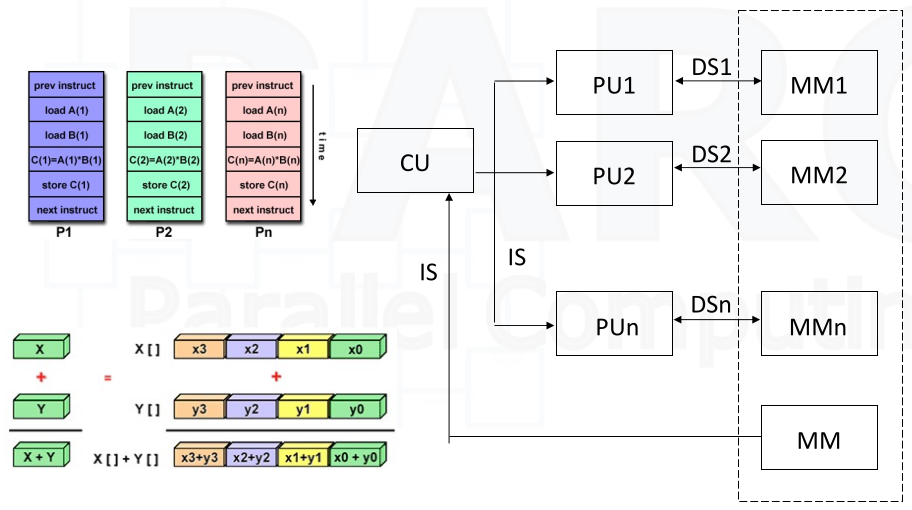
\includegraphics[width=\linewidth]{img/simd}
		\caption{simd.}
		\label{fig:simd}
	\end{subfigure}
	\hfill
	\begin{subfigure}{0.45\linewidth}
		\centering
		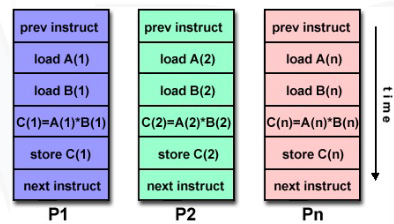
\includegraphics[width=\linewidth]{img/simd-processori}
		\caption{diversi processori eseguono la stessa istruzione su dati differenti.}
		\label{fig:simd-processori}
	\end{subfigure}
\end{figure}
SIMD è un tipo di parallel computer dove \textit{single istruction} significa che tutte le unità di elaborazione (PU) eseguono la stessa istruzione a ogni dato ciclo di clock. \textit{Multiple data} vuol dire che ogni unità di elaborazione (PU) può operare su un diverso elemento di dati. SIMD è più adatto per problemi specializzati
caratterizzati da un alto grado di
regolarità, come l'elaborazione di grafica/immagini. SIMD permette un esecuzione \textbf{deterministica} e \textbf{sincrona} (lockstep\footnote{Termine che ha origine militare, usato per riferirsi al passo sincronizzato dei soldati. In SIMD si riferisce all'esecuzione sincrona -- la CU non istruisce le PU se prima non è terminata l'elaborazione dell'istruzione precedente.}). La maggior parte dei computer moderni, in particolare quelli con unità di elaborazione grafica (GPU), impiegano istruzioni SIMD e unità di esecuzione.
\subsection*{MISD -- Multiple Instruction Single Data}

\begin{figure}[th]
	
	\begin{subfigure}{0.45\linewidth}
		\centering
		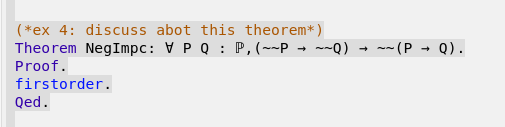
\includegraphics[width=\linewidth]{img/misd}
		\caption{misd.}
		\label{fig:misd}
	\end{subfigure}
	\hfill
	\begin{subfigure}{0.45\linewidth}
			\centering
		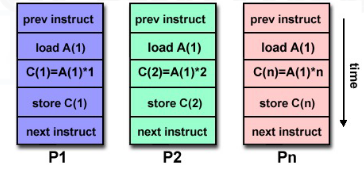
\includegraphics[width=0.7\linewidth]{img/misd-processori}
		\caption{le istruzioni sono diverse da processore a processore, ma il dato su cui operano è lo stesso.}
		\label{fig:misd-processori}		
	\end{subfigure}
\end{figure}
In MISD un singolo flusso di dati viene immesso in più unità di elaborazione. Ogni unità di elaborazione opera sui dati in modo indipendente tramite flussi di istruzioni indipendenti. Sono esistiti pochi esempi concreti di questa classe di computer paralleli. Uno è il computer sperimentale Carnegie-Mellon C.mmp (1971).

Alcuni possibili utilizzi potrebbero essere:
\begin{itemize}
	\item filtri di frequenza multipli che operano su un singolo flusso di segnale;
	\item algoritmi crittografici multipli che tentano di decifrare un singolo
	messaggio codificato.
\end{itemize}

\subsection*{MIMD -- Multiple Instruction Multiple Data}
\begin{figure}[th]
	\begin{subfigure}{0.45\linewidth}
		\centering
		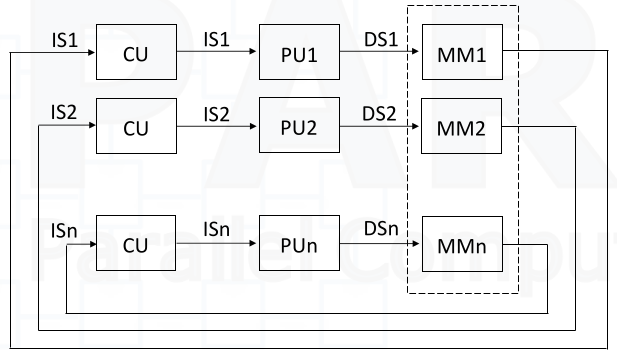
\includegraphics[width=\linewidth]{img/mimd}
		\caption{mimd.}
		\label{fig:mimd}
	\end{subfigure}
	\hfill
	\begin{subfigure}{0.45\linewidth}
		\centering
		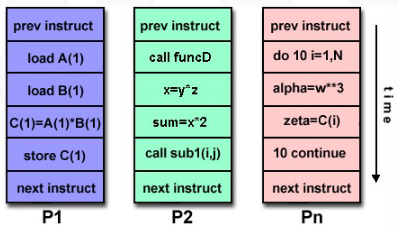
\includegraphics[width=\linewidth]{img/mimd-processori}
		\caption{istruzioni diverse vengono eseguite sui diversi processori che operano su dati differenti.}
		\label{fig:mimd-processori}
	\end{subfigure}
\end{figure}

Attualmente, il tipo più comune di computer parallelo. La maggior parte dei computer moderni rientra in questa categoria. \textit{Multiple Instruction} significa che ogni processore può eseguire un diverso flusso di istruzioni. \textit{Multiple Data} significa che ciascun processore può lavorare su un diverso flusso di dati. L'esecuzione può essere sincrona o asincrona, deterministica o non deterministica. MIMD viene utilizzata sulla maggior parte dei supercomputer attuali, cluster di computer paralleli in rete e \textit{"grid"}, computer SMP multiprocessore e PC multicore. Nota: molte architetture MIMD includono anche sottocomponenti di esecuzione SIMD.

\subsection{Terminologia delle architetture parallele}
\begin{itemize}
	\item \textbf{task}: una sezione logicamente discreta di
	lavoro computazionale. Un task è in genere un
	programma o un insieme di istruzioni simili a un programma che
	viene eseguito da un processore;
	\item \textbf{task parallelo}: un'attività che può essere eseguita da più processori in modo sicuro (produce risultati corretti);
	\item \textbf{esecuzione seriale}: esecuzione di un programma
	in sequenza, un'istruzione alla volta. Nel senso più semplice, questo è ciò che accade su una
	macchina con un solo processore. Tuttavia, praticamente tutte
	le attività parallele avranno sezioni di un programma parallelo che devono essere eseguite in serie;
	\item \textbf{esecuzione parallela}: esecuzione di un programma da parte di
	più di un task, con ogni task in grado
	di eseguire la stessa istruzione o un'istruzione diversa nello
	stesso momento;
	\item \textbf{pipelining}: suddividere un'attività in passaggi eseguiti
	da diverse unità di elaborazione, che prendono i vari flussi di input, proprio come avviene in una catena di montaggio; è un tipo di elaborazione parallela;
	\begin{figure}[th]
		\centering
		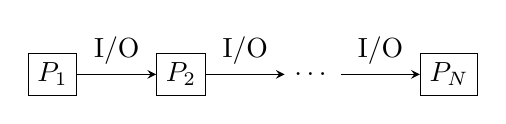
\begin{tikzpicture}
			\node[draw](A){$P_1$};
			\node[draw,right=of A](B){$P_2$};
			\node[right=of B](D){\dots};
			\node[draw, right=of D](C){$P_N$};
			\foreach \a/\b in {A/B,B/D,D/C}{
				\draw[-stealth,label distance=0.3pt, label=I/O] (\a)--(\b) node[pos=0.5,above]{I/O};
			}
		\end{tikzpicture}
		\label{fig:pipeline}
		\caption{pipeline.}
	\end{figure}
	\item \textbf{memoria condivisa}: da un punto di vista strettamente hardware, descrive un'architettura di computer
	in cui tutti i processori hanno accesso diretto (solitamente basato su bus) alla memoria fisica comune. In senso di programmazione, descrive un modello in cui
	i task paralleli hanno tutti la stessa "immagine" di
	memoria e possono indirizzare e accedere direttamente alle
	stesse posizioni di memoria logica indipendentemente da
	dove si trovi effettivamente la memoria fisica;
	\item \textbf{multiprocessore simmetrico (SMP)}: architettura hardware in cui più processori condividono un singolo spazio di indirizzamento e l'accesso a tutte le risorse; elaborazione a memoria condivisa;
	\item \textbf{memoria distribuita}: nell'hardware, si riferisce all'accesso alla memoria basato sulla rete per la memoria fisica che non è comune. Come modello di programmazione, le attività possono solo "vedere" logicamente la memoria della macchina locale e devono utilizzare le comunicazioni per accedere alla memoria su altre macchine in cui sono in esecuzione altre attività;
	\item \textbf{comunicazione}: le attività parallele in genere devono
	scambiare dati. Ci sono diversi modi per farlo,
	ad esempio tramite un bus di memoria condiviso
	o su una rete, tuttavia l'evento effettivo dello
	scambio di dati è comunemente definito come comunicazioni
	indipendentemente dal metodo impiegato;
	\item \textbf{sincronizzazione}: spesso è implementata stabilendo un punto di sincronizzazione all'interno di un'applicazione dove un'attività non può procedere ulteriormente finché un'altra attività (o più attività) non raggiunge lo stesso punto o un punto logicamente equivalente. La sincronizzazione di solito comporta l'attesa da parte di almeno un'attività, e quindi può causare un aumento del tempo di esecuzione totale dell'applicazione parallela;
	\item \textbf{granularità}: è una
	misura qualitativa del rapporto tra elaborazione e
	comunicazione;
	\begin{itemize}
		\item \textbf{coarse}: quantità relativamente grandi di lavoro computazionale vengono eseguite tra gli eventi di comunicazione;
		\item \textbf{fine}: quantità relativamente piccole di lavoro computazionale vengono eseguite tra gli eventi di comunicazione;
	\end{itemize}
	\item \textbf{speedup osservato}: è l'accelerazione osservabile nell'esecuzione di un codice che è stato parallelizzato ed è definito come
	\begin{equation*}
		\textsf{speedup}=\frac{\textsf{wall-clock time esecuzione seriale}}{\textsf{wall-clock time esecuzione parallela}}
	\end{equation*}
	Il \textit{wall-clock time} è la differenza tra il momento in cui un'attività termina e il momento in cui l'attività è iniziata.
	\item \textbf{overhead parallelo}: la quantità di tempo richiesta per
	coordinare attività parallele, anziché svolgere un lavoro
	utile. Il sovraccarico parallelo può includere fattori quali:
	\begin{itemize}
		\item tempo di avvio dell'attività;
		\item sincronizzazioni;
		\item comunicazioni dati;
		\item sovraccarico software imposto da compilatori paralleli, librerie,
		strumenti, sistema operativo, ecc;
		\item tempo di terminazione dell'attività;
	\end{itemize}
	\item \textbf{massivamente parallelo}: si riferisce all'hardware di un sistema parallelo che ha molti processori;
	\item \textbf{parallelizzazione embarassingly}: risolve contemporaneamente molti compiti simili, ma indipendenti. C'è poca o nessuna necessità di coordinamento tra i compiti;
	\item \textbf{scalabilità}: si riferisce alla capacità di un sistema parallelo (HW e/o SW)
	di dimostrare un aumento proporzionale dell'accelerazione parallela
	con l'aggiunta di più processori. I fattori che contribuiscono alla
	scalabilità includono:
	\begin{itemize}
		\item hardware, in particolare larghezze di banda memoria-CPU e comunicazioni di rete;
		\item algoritmo applicativo;
		\item sovraccarico parallelo correlato;
		\item caratteristiche dell'applicazione specifica e della codifica;
	\end{itemize}
	\item \textbf{processori multicore}: più processori (core) su un singolo
	chip;
	\item \textbf{cluster computing}: utilizzo di una combinazione di unità di base
	(processori, reti o SMP) per costruire un sistema parallelo;
	\item \textbf{supercomputing/ high performance computing}: l'uso delle macchine più veloci e grandi del mondo per risolvere grandi problemi;
	\item \textbf{edge computing}: paradigma di elaborazione distribuita che avvicina il calcolo e l'archiviazione dei dati alla posizione in cui sono necessari, per migliorare i tempi di risposta e risparmiare larghezza di banda;
\end{itemize}

\subsection{Shared memory}I computer paralleli a memoria condivisa variano molto, ma generalmente hanno in comune
la capacità di tutti i processori di accedere a tutta la memoria come spazio di indirizzamento globale.


Più processori possono operare indipendentemente ma condividere le stesse
risorse di memoria. Le modifiche in una posizione di memoria effettuate da un processore sono visibili a tutti
gli altri processori. 

Le macchine a memoria condivisa possono essere divise in due classi principali in base ai tempi di accesso alla memoria: UMA e NUMA.
\subsubsection{UMA}
\begin{figure}[th]
	\centering
	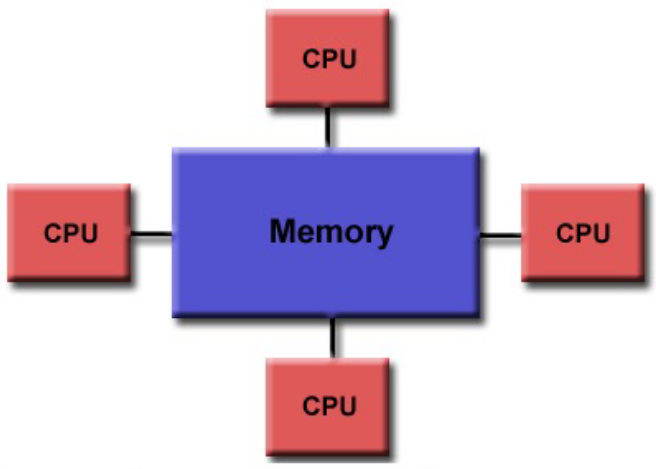
\includegraphics[width=0.7\linewidth]{img/shared-memory}
	\caption{shared memory classe UMA.}
	\label{fig:shared-memory}
\end{figure}
Uniform Memory Access (UMA): oggi più comunemente rappresentato da Macchine Symmetric
Multiprocessor (SMP). I processori sono identici, i tempi di accesso e il modo in cui si accede alla memoria sono gli stessi. A volte chiamato \textbf{CC-UMA (Cache Coherent UMA)}. \textit{Cache coherent} significa che se un processore aggiorna una posizione nella memoria condivisa, tutti gli altri processori sono a conoscenza dell'aggiornamento. La cache coherent è realizzata a livello hardware.
\subsubsection{NUMA}
\begin{figure}[th]
	\centering
	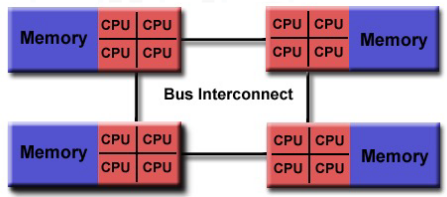
\includegraphics[width=0.7\linewidth]{img/numa}
	\caption{shared memory classe NUMA.}
	\label{fig:numa}
\end{figure}
L'accesso alla memoria non uniforme (NUMA) viene spesso realizzato collegando fisicamente due o più SMP. Un SMP può accedere direttamente alla memoria di un altro SMP. Non tutti i processori hanno lo stesso tempo di accesso a tutte le memorie. L'accesso alla memoria attraverso il collegamento è più lento. Se viene mantenuta la coerenza della cache, può anche essere chiamato \textbf{CC-NUMA --
Cache Coherent NUMA}.
\subsection{Vantaggi e svantaggi delle memorie condivise}
\subsubsection*{Vantaggi}
\begin{itemize}
	\item Lo spazio di indirizzamento globale fornisce una prospettiva di programmazione user-friendly
	per la memoria.
	\item La condivisione dei dati tra le attività è veloce e uniforme grazie alla
	prossimità della memoria alle CPU.
\end{itemize}
\subsubsection*{Svantaggi}
\begin{itemize}
	\item Lo svantaggio principale è la mancanza di scalabilità tra memoria e
	CPU: aggiungere più CPU può aumentare geometricamente il traffico sul percorso memoria-CPU condiviso e, per i sistemi cache coerenti, aumentare geometricamente il traffico associato alla gestione cache/memoria.
	\item  La responsabilità ricade sul programmatore che deve utilizzare i costrutti di sincronizzazione i quali assicurano
	un accesso "corretto" alla memoria globale.
	\item  Diventa sempre più difficile e costoso progettare e
	produrre macchine a memoria condivisa con un numero sempre maggiore di
	processori.
\end{itemize}
\clearpage
\subsection{Memoria distribuita}
\begin{figure}[th]
	\centering
	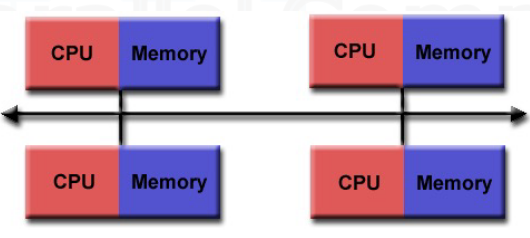
\includegraphics[width=0.7\linewidth]{img/memoria-distribuita}
	\caption{memoria distribuita.}
	\label{fig:memoria-distribuita}
\end{figure}
I sistemi di memoria distribuita richiedono una rete di comunicazione per connettere la memoria interprocessore. I processori hanno la loro memoria locale. Gli indirizzi di memoria in un processore non sono mappati su un altro processore, quindi non esiste un concetto di spazio di indirizzamento globale tra tutti i processori. Poiché ogni processore ha la propria memoria locale, funziona
indipendentemente. Le modifiche apportate alla memoria locale non hanno
effetto sulla memoria di altri processori. Quindi, \textbf{il concetto di
coerenza della cache non si applica}.
Quando un processore ha bisogno di accedere ai dati in un altro processore,
di solito è compito del programmatore definire esplicitamente come
e quando i dati vengono comunicati. Anche la sincronizzazione tra le attività
è responsabilità del programmatore.
La rete utilizzata per il trasferimento dei dati varia ampiamente,
anche se può essere formata da semplici collegamenti Ethernet.

\subsubsection*{Vantaggi}
\begin{itemize}
	\item La memoria è scalabile con il numero di processori. Aumentando il numero di processori, la dimensione della memoria aumenta proporzionalmente. 
	\item Ogni processore può accedere rapidamente alla propria memoria senza
	interferenze e senza il sovraccarico sostenuto nel tentativo di
	mantenere la coerenza della cache.
	\item Efficienza dei costi: può utilizzare processori e reti commerciali e off-the-shelf.
\end{itemize}
\subsubsection*{Svantaggi}
\begin{itemize}
	\item Il programmatore è responsabile di molti dei dettagli associati alla comunicazione dati tra processori.
	\item Potrebbe essere difficile mappare le strutture dati esistenti, basate sulla memoria globale, a questa organizzazione della memoria.
	\item Tempi di accesso alla memoria non uniforme (NUMA).
\end{itemize}
\clearpage
\subsection{Memoria distribuita ibrida}
\begin{figure}[th]
	\centering
	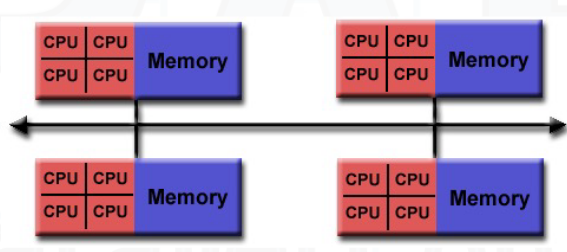
\includegraphics[width=0.7\linewidth]{img/memoria-distribuita-ibrida}
	\caption{memoria distribuita ibrida.}
	\label{fig:memoria-distribuita-ibrida}
\end{figure}
I computer più grandi e veloci del mondo oggi impiegano sia architetture di memoria condivisa che distribuita. Il componente di memoria condivisa è solitamente una macchina SMP coerente con la cache. I processori su un dato SMP possono indirizzare la memoria di quella macchina come globale. Il componente di memoria distribuita è la rete di più SMP.
Gli SMP conoscono solo la propria memoria, non quella di un altro
SMP. Pertanto, sono necessarie comunicazioni di rete per spostare i dati da
un SMP all'altro.
 Le tendenze attuali sembrano indicare che questo tipo di architettura di memoria continuerà a prevalere e ad aumentare nella fascia alta dell'informatica, probabilmente anche in futurp.
\subsubsection*{Vantaggi e svantaggi}Qualunque cosa sia comune sia alle architetture di memoria condivisa che a quelle distribuite.

\section{Modelli di programmazione parallela}
Esistono diversi modelli di programmazione parallela di uso comune.
\subsection{Panoramica}
Sebbene possa non sembrare ovvio, questi modelli non sono
specifici per un particolare tipo di macchina o architettura di memoria. Infatti, uno qualsiasi di questi modelli può (teoricamente)
essere implementato su qualsiasi hardware sottostante. Due esempi:
\begin{enumerate}
	\item  Modello di \textbf{memoria condivisa} su una macchina a \textbf{memoria distribuita}:
	\begin{itemize}
		\item  Approccio ALLCACHE di Kendall Square Research (KSR). La memoria della macchina era distribuita fisicamente, ma appariva all'utente come una
		singola memoria condivisa (spazio di indirizzamento globale). In genere, questo
		approccio è definito "memoria condivisa virtuale".
	\end{itemize}
	\item  Modello di \textbf{passaggio di messaggi} su una macchina a \textbf{memoria condivisa}:
	\begin{itemize}
		\item  MPI su SGI Origin. SGI Origin ha impiegato il tipo  di
		architettura di memoria condivisa CC-NUMA, in cui ogni attività ha accesso diretto alla
		memoria globale. Tuttavia, la capacità di inviare e ricevere messaggi
		con MPI, come avviene comunemente su una rete di macchine a memoria distribuita, non è solo implementata, ma è anche molto
		utilizzata.
	\end{itemize}
\end{enumerate}
\subsection{Modello shared memory}
Nel modello di programmazione a memoria condivisa, le attività condividono uno spazio di indirizzamento comune, che leggono e scrivono in modo asincrono. Vari meccanismi come blocchi/semafori possono essere utilizzati per controllare l'accesso alla memoria condivisa. Un vantaggio di questo modello dal punto di vista del programmatore è che manca la nozione di "proprietà" dei dati. Non c'è bisogno di specificare esplicitamente la comunicazione dei dati tra le attività. Lo sviluppo del programma spesso può essere semplificato. Uno svantaggio importante in termini di prestazioni è che diventa più difficile comprendere e gestire la località dei dati. Mantenere i dati locali al processore che li elabora conserva gli accessi alla memoria, gli aggiornamenti della cache e il traffico del bus che si verifica quando più processori utilizzano gli stessi dati. Sfortunatamente, il controllo della località dei dati è difficile da comprendere e al di fuori del controllo dell'utente medio.
\subsubsection*{Implementazione}
Nelle piattaforme a memoria condivisa, i compilatori nativi
traducono le variabili del programma utente in indirizzi di memoria effettivi, che sono globali.
Attualmente non esistono implementazioni comuni di piattaforme a memoria distribuita. Tuttavia, come menzionato in precedenza nella sezione Panoramica,
l'approccio KSR ALLCACHE ha fornito una vista di memoria condivisa dei dati, anche se la memoria fisica della
macchina era distribuita.
\subsection{Modello delle threads}

Nel modello di programmazione parallela dei thread, un singolo processo può avere più percorsi di esecuzione simultanei. Forse l'analogia più semplice che può essere utilizzata per descrivere le thread è il concetto di un singolo programma che include un certo numero di subroutine:
\begin{figure}[th]
	\centering
	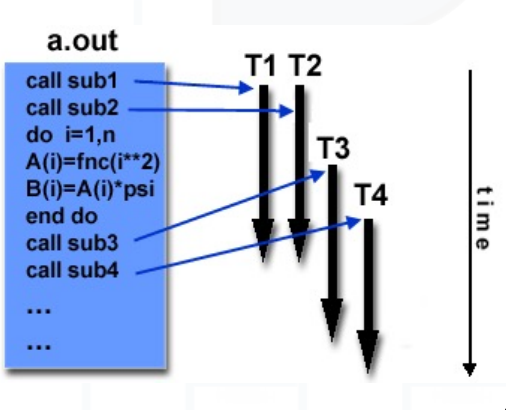
\includegraphics[width=0.4\linewidth]{img/modello-thread}
	\caption{modello delle thread.}
	\label{fig:modello-thread}
\end{figure}

\begin{itemize}
	\item Il programma principale a.out è programmato per essere eseguito dal sistema operativo nativo. a.out carica
	e acquisisce tutte le risorse di sistema e utente necessarie per l'esecuzione.
	\item a.out esegue un lavoro seriale e quindi crea un certo numero di attività
	(thread) che possono essere programmate ed eseguite dal sistema operativo contemporaneamente.
	\item Ogni thread ha dati locali, ma condivide anche tutte le risorse di a.out.
	Ciò consente di risparmiare il sovraccarico associato alla replica delle risorse di un programma
	per ogni thread. Ogni thread trae vantaggio anche da una vista della memoria globale
	perché condivide lo spazio di indirizzamento di a.out.
	\item Il lavoro di una thread può essere descritto al meglio come una subroutine all'interno del programma
	principale. Qualsiasi thread può eseguire qualsiasi subroutine contemporaneamente ad altre thread. 
	\item Le thread comunicano tra loro tramite la memoria globale (aggiornando
	le posizioni degli indirizzi). Ciò richiede costrutti di sincronizzazione per garantire che
	più di una thread non stia aggiornando lo stesso indirizzo globale in qualsiasi
	momento.
	\item Le thread possono andare e venire, ma a.out rimane presente per fornire le risorse necessarie condivise
	fino al completamento dell'applicazione.
\end{itemize}
\subsubsection*{Implementazione}
Le thread sono comunemente associate alle architetture di memoria condivisa e ai sistemi operativi.
Da una prospettiva della programmazione, le implementazioni delle thread comunemente
comprendono:
\begin{itemize}
	\item una libreria di subroutine che vengono chiamate dall'interno del codice sorgente parallelo;
	\item un set di direttive del compilatore incorporate nel codice sorgente seriale o parallelo.
\end{itemize}
In entrambi i casi, il programmatore è responsabile della determinazione di tutto
il parallelismo.
Le implementazioni delle thread non sono una novità nell'informatica.
 Storicamente, i fornitori di hardware hanno implementato le proprie
versioni proprietarie di thread.
 Queste implementazioni differivano sostanzialmente l'una dall'altra, rendendo
difficile per i programmatori sviluppare applicazioni thread portatili.
Sforzi di standardizzazione non correlati hanno portato a due implementazioni di thread molto diverse:
 \begin{enumerate}
 	\item thread POSIX;
 	\item OpenMP.
 \end{enumerate}
 
 \subsubsection{Thread POSIX}
 Basato su libreria;
  richiede codifica parallela.
 Specificato dallo standard IEEE POSIX 1003.1c (1995).
 Solo linguaggio C.
 Comunemente noto come Pthread.
 La maggior parte dei fornitori di hardware ora offre Pthread oltre
 alle loro implementazioni di thread proprietarie.
 Parallelismo molto esplicito;
  richiede una notevole attenzione ai dettagli da parte del programmatore.
  
  \subsubsection{OpenMP}
  Basato su direttiva del compilatore;
   può usare codice seriale.
  Definito congiuntamente e approvato da un gruppo di importanti fornitori di hardware e software per computer.
   L'API Fortran OpenMP è stata rilasciata il 28 ottobre 1997.
   L'API C/C++ è stata rilasciata alla fine del 1998.
  Portabile/multipiattaforma, incluse le piattaforme Unix e Windows NT
  Disponibile nelle implementazioni C/C++ e Fortran
  Può essere molto facile e semplice da usare - fornisce
  "parallelismo incrementale". Microsoft ha la sua implementazione per i thread, che non è correlata allo standard UNIX POSIX o OpenMP.
  
\subsection{Modello di passaggio dei messaggi}
\begin{figure}[th]
	\centering
	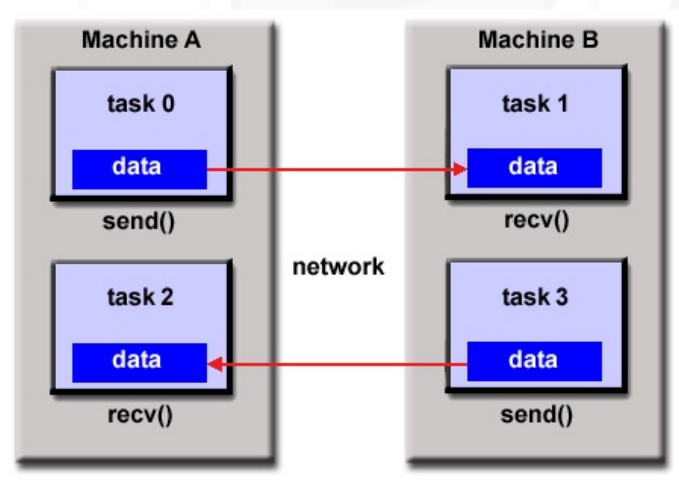
\includegraphics[width=0.7\linewidth]{img/modello-di-passaggio-dei-messaggi}
	\caption{modello di passaggio dei messaggi.}
	\label{fig:modello-di-passaggio-dei-messaggi}
\end{figure}

Il modello di passaggio dei messaggi dimostra le seguenti
caratteristiche:
\begin{itemize}
	
	\item un set di attività che utilizzano la propria
	memoria locale durante il calcolo. Più
	attività possono risiedere sulla stessa
	macchina fisica e anche su un numero arbitrario
	di macchine;
	\item le attività scambiano dati tramite
	comunicazioni inviando e
	ricevendo messaggi;
	\item il trasferimento dei dati richiede solitamente
	che ogni processo esegua
	operazioni cooperative. Ad esempio, un'operazione di invio
	deve avere un'operazione di ricezione
	corrispondente.
\end{itemize}
\subsubsection*{Implementazione}
Da una prospettiva di programmazione, le implementazioni di passaggio di messaggi
comprendono comunemente una libreria di
subroutine che sono incorporate nel codice sorgente.
 Il programmatore è responsabile della determinazione di tutto
il parallelismo.
Storicamente, una varietà di librerie di passaggio di messaggi
sono state disponibili fin dagli anni '80.
 Queste implementazioni differivano sostanzialmente
l'una dall'altra, rendendo difficile per i programmatori sviluppare
applicazioni portabili.
Nel 1992, è stato formato il MPI Forum con l'obiettivo primario di stabilire un'interfaccia standard per le implementazioni di passaggio di messaggi.

MPI è ora lo standard industriale "de facto" per il passaggio di messaggi,
sostituendo praticamente tutte le altre implementazioni di passaggio di messaggi utilizzate
per il lavoro di produzione.
 La maggior parte, se non tutte, delle piattaforme di elaborazione parallela più diffuse offrono almeno
un'implementazione di MPI. Alcune offrono un'implementazione completa di MPI-2.
Per le architetture a memoria condivisa, le implementazioni MPI di solito non
utilizzano una rete per le comunicazioni delle attività. Utilizzano la memoria condivisa
(copie di memoria) per motivi di prestazioni.
\subsection{Modello parallelo dei dati}
\begin{figure}[th]
	\centering
	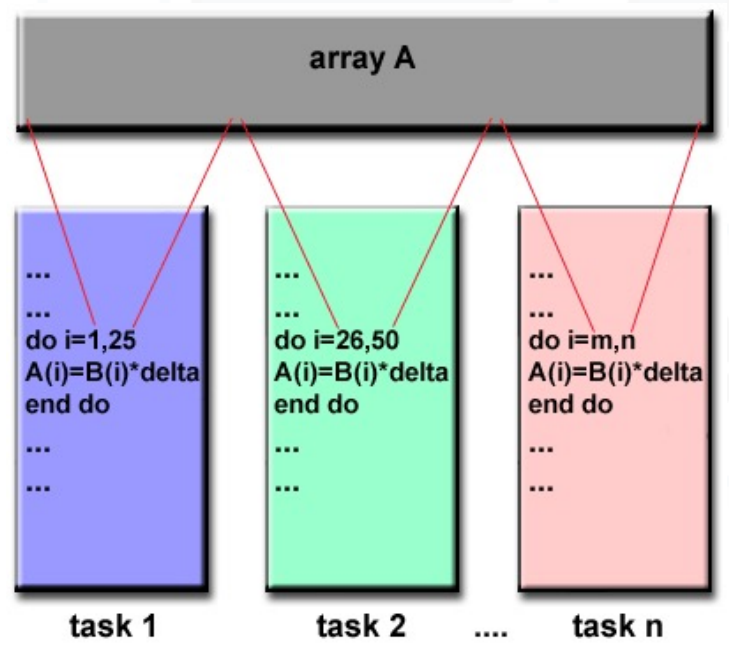
\includegraphics[width=0.7\linewidth]{img/modello-parallelo-dei-dati}
	\caption{modello parallelo dei dati.}
	\label{fig:modello-parallelo-dei-dati}
\end{figure}

Il modello parallelo di dati dimostra le seguenti caratteristiche:
\begin{itemize}
	\item La maggior parte del lavoro parallelo si concentra
	sull'esecuzione di operazioni su un set di dati.
	Il set di dati è in genere organizzato in
	una struttura comune, come un array
	o un cubo.
	\item Un set di attività lavora collettivamente sulla
	stessa struttura di dati, tuttavia, ogni
	attività lavora su una partizione diversa della
	stessa struttura di dati.
	\item Le attività eseguono la stessa operazione sulla
	loro partizione di lavoro, ad esempio,
	"aggiungi 4 a ogni elemento dell'array".
\end{itemize}
Nelle architetture a memoria condivisa, tutti i task possono avere accesso alla
struttura dati tramite memoria globale. Nelle architetture a memoria distribuita, la struttura dati è suddivisa e risiede come "blocchi"
nella memoria locale di ciascun task.
\subsubsection*{Implementazione}
La programmazione con il modello parallelo di dati viene solitamente eseguita scrivendo un programma con costrutti paralleli di dati. I costrutti possono essere chiamate a una libreria di subroutine parallele di dati o direttive del compilatore riconosciute da un compilatore parallelo di dati.
\subsection{Modello ibrido}	È una combinazione dei modelli presentati precedentemente. Ad esempio:
\begin{itemize}
	\item combinazione del modello di passaggio dei messaggi con con il modello delle thread (thread POSIX) o il modello di memoria condivisa (OpenMP);
	\item combinazione del modello dei dati paralleli con il modello di passaggio dei messaggi.
\end{itemize}
\subsection{Modello SPMD -- Single Program Multiple Data}
\begin{figure}[th]
	\centering
	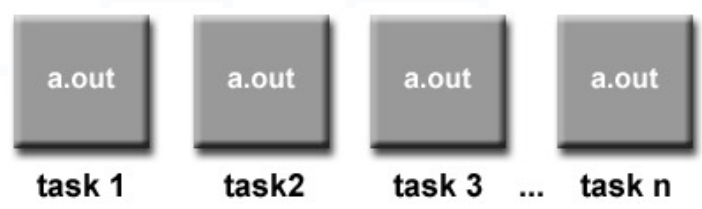
\includegraphics[width=0.7\linewidth]{img/spmd}
	\caption{modello SPMD.}
	\label{fig:spmd}
\end{figure}

SPMD è in realtà un modello di programmazione "di alto livello" che può essere costruito
su qualsiasi combinazione dei modelli di programmazione parallela menzionati in precedenza.
Un singolo programma viene eseguito da tutte le attività simultaneamente.
In qualsiasi momento, le attività possono eseguire le stesse o diverse
istruzioni all'interno dello stesso programma.
\subsubsection*{SPMD vs SIMD}
In SPMD, più processori autonomi eseguono simultaneamente lo stesso
programma in punti indipendenti, anziché nel lockstep che SIMD impone
su dati diversi.
 Con SPMD, le attività possono essere eseguite su CPU per uso generale; SIMD richiede
processori vettoriali per manipolare flussi di dati.
 SPMD è una sottocategoria di MIMD.
I programmi SPMD di solito hanno la logica necessaria programmata al loro interno per
consentire a diverse attività di ramificarsi o eseguire in modo condizionale solo quelle parti del
programma che sono progettate per eseguire. Vale a dire, le attività non devono necessariamente
eseguire l'intero programma, forse solo una parte di esso.
Tutte le attività possono utilizzare dati diversi.
\subsection{Modello MPMD -- Multiple Program Multiple Data} 
\begin{figure}[th]
	\centering
	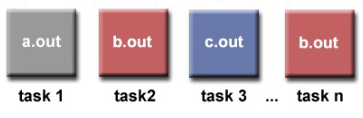
\includegraphics[width=0.7\linewidth]{img/mpmd}
	\caption{modello MPMD.}
	\label{fig:mpmd}
\end{figure}

Come SPMD, MPMD è in realtà un modello di programmazione "di alto livello" che
può essere costruito su qualsiasi combinazione dei modelli di programmazione parallela menzionati in precedenza.
Le applicazioni MPMD in genere hanno più file oggetto eseguibili
(programmi). Mentre l'applicazione viene eseguita in parallelo, ogni attività
può eseguire lo stesso programma o un programma diverso rispetto ad altre attività.
Tutte le attività possono utilizzare dati diversi.
	\section{Valutazione delle performance}
La valutazione delle performance viene fatta per due motivi:
\begin{itemize}
    \item dal punto di vista dell'\textbf{utente} per ridurre il tempo di risposta. È nota anche come \textbf{tempo di esecuzione} o \textbf{latenza}. Definita come il tempo trascorso dall'inizio al completamento del compito o lavoro;

\item dal punto di vista del \textbf{sistema} per aumentare il \textbf{throughput}, ovvero la quantità totale di lavoro svolto in un dato intervallo di tempo, a volte chiamato \textbf{larghezza di banda}.

\end{itemize}

Lo speedup è definito come il rapporto tra il tempo di esecuzione di due programmi:
\begin{equation*}
	n=\frac{execTime_y}{execTime_x}
	=\frac{\frac{1}{\textsc{Performance}_y}}{\frac{1}{\textsc{Performance}_x}}=\frac{\textsc{Performance}_x}{\textsc{Performance}_y}
\end{equation*}
e misura il miglioramento delle prestazioni. \textbf{Nota:} il tempo di esecuzione è \textit{inversamente proporzionale} alle performance. Di solito $execTime_y$ viene sostituito dal tempo di esecuzione della versione sequenziale di un programma $P$ e $execTime_x$ con la sua versione parallelizzata.

Le misurazioni delle performance possono essere fatte a diversi livelli (considerando solo l'architettura hardware, una sua parte, o una parte di codice, o un intero programma, oppure tutto l'insieme) sfruttando funzionalità contenute in una \textbf{benchmark suite} (un insieme di tool di benchmark, come i \textbf{kernels} che sono piccoli pezzi di codice chiave presi da applicazioni reali, oppure i \textbf{toy programs} che contengono programmi, solitamente lunghi 100 linee di codice, che implementano algoritmi come la moltiplicazione tra matrici, il quicksort, e così via. Vi sono poi i \textbf{benchmark sintetici}, ovvero programmi ideati per simulare il comportamento delle applicazioni reali (come il Linpak, e il Dhrystone). La \textbf{SPEC} (Standard Performance Evaluation Corporation) è un consorzio senza scopo di lucro che stabilisce, mantiene e approva benchmark e strumenti standardizzati per valutare le prestazioni per la nuova generazione di sistemi informatici. SPEC sviluppa suite di benchmark e inoltre esamina e pubblica i risultati presentati dalle nostre organizzazioni membri e da altri licenziatari di benchmark.

Per comparare le performance di un componente hardware può essere consultata una \textbf{tabelle delle performance} dei modelli disponibili in commercio. Le informazioni più importanti riguardano i benchmark per completare un particolare task e il costo del componente hardware.

\subsection{Principio quantitativo} Per aumentare lo speedup è necessario concentrare le energie sul codice che viene eseguito più frequentemente, piuttosto che quello eseguito più raramente.

Un importante riferimento a tal proposito, è la \textbf{legge di Amdahl}.

\vspace{.5cm}
\begin{tcolorbox}[title=Legge di Amdahl]
    \textit{"Il miglioramento delle prestazioni di un sistema che si può ottenere ottimizzando una certa parte del sistema è limitato dalla frazione di tempo in cui tale parte è effettivamente utilizzata"}.
\end{tcolorbox}
\vspace{.5cm}

\subsubsection*{Legenda}
\begin{table}[th]
	\centering
	\begin{tblr}{|c|c|}
		\hline
		$e_n$ & execution time new
		\\\hline
		$e_o$ & execution time old
		\\\hline
		$f_i$ & fraction improved
		\\\hline
		$s_i$ & speedup improved
		\\\hline
		$s_g$ & speedup global
		\\\hline
	\end{tblr}
\end{table}

Di seguito con $f_i \le 1$ (\textit{"fraction improved"}) viene indicata la frazione del tempo di esecuzione della macchina originale (o del codice originale) che può essere modificata per trarre vantaggio dalle migliorie, mentre con $s_i \ge 1$ (\textit{"speedup improved"}) viene indicato il miglioramento ottenuto da un una modalità di esecuzione più veloce.
\begin{align}
    e_n &= e_o \cdot \left((1-f_i) + \frac{f_i}{s_i} \right) \label{eqn:execution-time-new} \\
    s_g &= \frac{e_o}{e_n}= \frac{1}{(1-f_i)+ \frac{f_i}{s_i}}\label{eqn:speedup-global}
\end{align}
Se un miglioramento può essere usato solo per una frazione dell'intero task:
\begin{equation}
    s_g = \frac{1}{(1-f_i)+\frac{f_i}{s_i}} \fcolorbox{red}{white}{$\le \frac{1}{(1-f_i)}$} \label{eqn:speedup-global-with-limit}
\end{equation}


Lo \textbf{speedup globale} $s_g$ è uguale a $ \frac{1}{(1-f_i)+\frac{f_i}{s_i}}$ dove $1-f_i$ è la frazione non parallelizzabile, $f_i$ è la frazione parallelizzabile e $s_i$ è lo speedup che si ottiene dalla porzione parallelizzabile di codice. Lo speedup globale massimo, nel riquadro rosso (equazione \ref{eqn:speedup-global-with-limit}) si ottiene facendo tendere la $s_i$ all'infinito: \[\lim_{s_i \to \infty}{\frac{f_i}{s_i}} = 0\]
\begin{exercise}
	Si consideri un miglioramento di 10 volte più veloce della macchina originale (o del codice) ma che può essere applicato solo per il 40\% del tempo. Qual'è il guadagno totale?
\end{exercise}
\begin{solution}
	Traendo i dati dal problema, si ottiene che lo $s_i = 10$ e che $f_i = 40\% = 0,4$. Sostituendo alla formula \ref{eqn:speedup-global} si ottiene
	\begin{equation*}
		s_g = \frac{1}{(1-0.4)+\frac{0.4}{10}} = \frac{1}{0.6+0.04} = \frac{1}{0.64} = \frac{100}{64} = 1.56
	\end{equation*}

	Lo speedup ottenuto è di 1.56.
\end{solution}

\begin{exercise}
	Si consideri una CPU che è stata aggiornata per avere i seguenti cambiamenti:
	\begin{enumerate}
		\item aumentare la velocità di un fattore pari a 5 senza interessare le performance del sistema I/O;
		\item il costo è 5 volte superiore al precedente;
		\item la CPU può essere utilizzata per il 50\% del tempo totale, mentre il rimanente viene impiegato per operazioni di I/O;
		\item il costo della CPU è $\frac{1}{3}$ del costo della macchina.
	\end{enumerate}
	Questo investimento, è conveniente?
\end{exercise}
\begin{solution}
	Lo $s_i = 5$, la $f_i = 50\% = 0.5$. Lo speedup globale è:
	\begin{equation*}
		s_g = \frac{1}{(1-0.5)+\frac{0.5}{5}}=\frac{1}{0.5+0.1} = \frac{10}{6} = 1.67
	\end{equation*}
	il costo è aumentato di:
	\begin{equation*}
		c = 1 \cdot \frac{2}{3} + 5 \cdot \frac{1}{3} =\frac{7}{3} = 2.33
	\end{equation*}
	Dato che il costo è superiore al rendimento ottenuto $ c = 2.33 >  s_g = 1.67 $ non è conveniente fare l'aggiornamento del processore.
\end{solution}

\begin{exercise}
	Si vuole riscrivere un programma su un'architettura MIMD con 100 processori. L'obbiettivo è di ridurre il tempo di esecuzione di 80 volte rispetto a quello precedente su un'architettura SISD. Qual'è la frazione del programma originale che può restare sequenziale?
\end{exercise}
\begin{solution}
	L'impostazione del problema è diversa dai precedenti. Il tempo di esecuzione della soluzione parallela è 80 volte più veloce di quella sequenziale. Si può osservare che il tempo totale è dato dalla somma del tempo di esecuzione della parte sequenziale e di quella parallela.
	\begin{align*}
		T&=\frac{T_{\textsc{sisd\textsubscript{\textsc{par}}}}}{\#\textsc{processori}}+\textsc{T\textsubscript{SISD}\textsubscript{\textsc{nonpar}}}\\
		&=\frac{T\textsubscript{\textsc{sisd}}\cdot \%\textsc{par}}{\#\textsc{processori}}+T_\textsc{sisd}\cdot\underbrace{ (1-\% par) }_{\%\textsc{nonpar}}
	\end{align*}
	La percentuale parallelizzabile è dell' $80\%$ rispetto al tempo iniziale ($T_\textsc{SISD}$).  Il numero di processori è $100$. Per semplicità si imposta ad $x=\% par$, ovvero la percentuale cercata.
	Sostituendo i dati nella formula:
	\begin{align*}
		\frac{\cancel{T_\textsc{sisd}}}{80}&=T_{\cancel{\textsc{sisd}}}\cdot \left(\frac{x}{100}+\underbrace{(1-x)}_{\textsc{\% nonpar}}\right)\\
		\frac{1}{80} &=  \frac{x}{100} + (1-x)\implies \frac{x+100-100\, x}{100}=\frac{1}{80}
		 \\ &\implies x = \left(\frac{5}{4}-100\right)\cdot\frac{1}{-99}\implies x = \frac{-395}{4}\cdot \frac{1}{-99}=0.997\\ &\implies x = 99.7\%
	\end{align*}
\end{solution}

\begin{exercise}
	Sapendo che il calcolo parallelo è 20 volte più veloce rispetto all'originale (sequenziale), calcolare:
	\begin{itemize}
		\item  la percentuale di parallelismo è la porzione di tempo impiegata utilizzando la modalità di esecuzione SIMD.
		\item Disegna un grafico per rappresentare il miglioramento delle prestazioni come percentuale del calcolo eseguito in modalità SIMD.
		\item  Quale percentuale di parallelismo è necessaria per ottenere un miglioramento delle prestazioni pari a 2? Quale per raggiungere la metà del miglioramento massimo?
	\end{itemize}
\end{exercise}
\begin{solution}
	Lo speedup che si ottiene è il seguente. Si pone $x=\% par$
	\begin{align*}
		\textsc{speedup} = \frac{1}{(1-x)+\frac{x}{\text{speedup par.}}} = \frac{1}{(1-x)+\frac{x}{20}} = \frac{20}{20-19 \, x}
	\end{align*}
	Il grafico è il seguente.
	\begin{figure}[ht]
		\centering
		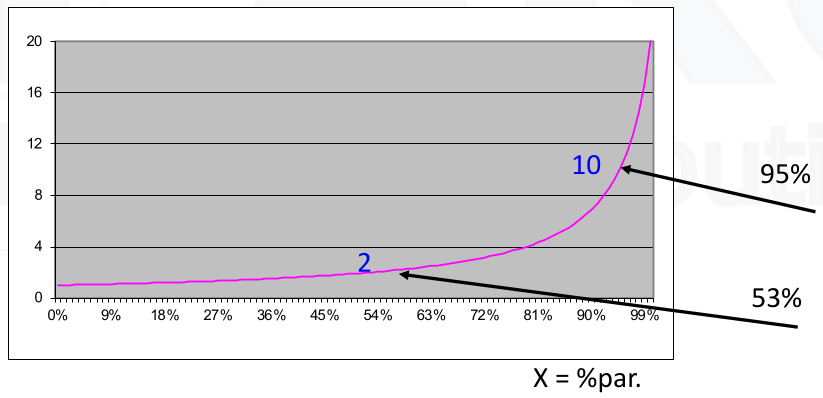
\includegraphics[width=0.7\linewidth]{img/graph-ex4}
		\caption{grafico dello speedup.}
		\label{fig:graph-ex4}
	\end{figure}
\end{solution}
Si consideri ora lo stesso esercizio ma con questi dati.
\begin{exercise}
	La percentuale di parallelismo raggiungibile è del 70\%. Ci sono due alternative.
	\begin{enumerate}
		\item Raddoppiare la velocità della modalità SIMD (è molto costoso)
		\item Aumentare la percentuale di parallelismo concentrandosi sul compilatore.
	\end{enumerate}
	Quale \textbf{aumento} della percentuale di parallelismo è necessario per ottenere lo stesso guadagno di prestazioni?
\end{exercise}
\begin{solution}
	Lo speedup originale si ottiene facendo
	\begin{equation*}
		\textsc{speedup orig}[20 \cdot 70 \%] = \frac{1}{(1-0.7)+\frac{0.7}{20}} = \frac{20}{20-14+0.7}=2.9851
	\end{equation*}
	Raddoppiando la velocità della modalità SIMD
	\begin{equation*}
		\textsc{speedup hw}[20 \cdot 70\%] = \frac{1}{(1-0.7)+\frac{0.7}{40}}=\frac{40}{40-28+0.7}=3.1496
	\end{equation*}
	Lo speedup adottando il compilatore è ovviamente parametrico, perché ci si sta chiedendo quale sia la percentuale necessaria per ottenere lo stesso guadagno di prestazioni, ed è il seguente.
	\begin{equation*}
		\textsc{speedup compiler}[20\cdot x\%] = \frac{1}{(1-x)+\frac{x}{20}}=\frac{20}{20-19\, x}
	\end{equation*}
	Si pone dunque
	\[\textsc{speedup compiler}= \textsc{speedup hw}\]
	ovvero
	\begin{equation*}
		\frac{20}{20-19\, x} = 3.1496 \implies x = 0.7184
	\end{equation*}
	Dunque è sufficiente una parallelizzazione del 71.84\%.
\end{solution}
\begin{exercise}
	Si consideri un'architettura basata su cache. La memoria cache è 5 volte più veloce della memoria principale. La cache è usata per il 90\% del tempo. Ci si chiede quale sia lo speedup con e senza cache.
\end{exercise}
\begin{solution}
	Lo speedup è il seguente.
	\begin{equation*}
		\textsc{speedup} = \frac{1}{(1-x)+\frac{x}{\textsc{speedup con cache}}} = \frac{1}{(1-0.9)+\frac{0.9}{5}}=\frac{1}{0.28}\approx 3.6
	\end{equation*}
	Si conclude che l'architettura basata su cache è più veloce di 3.6 volte la velocità della stessa architettura senza cache.
\end{solution}
%%%%%%%%%%%%%%%%%%%%%%%%%%%%%%%%%%%%%%%%%%%%%%%%%%%%%%%%%%%%%%%%%%%%%%%%

\subsection{Tempo di esecuzione} Il tempo di esecuzione viene usato per misurare le performance di un computer: l'architettura che esegue la stessa quantità di lavoro in meno tempo è la più veloce. Il \textbf{tempo di risposta} rappresenta la latenza per completare un task e include accessi al disco, gli accessi alla memoria e le operazioni di input/output. Il \textbf{CPU time} ovvero il tempo impiegato per svolgere operazioni di CPU (cicli di clock per eseguire il codice interessato, per operazioni di sistema -- ad esempio per la stampa a video -- mentre non è considerato CPU time il tempo speso per attendere dati o istruzioni accedendo in memoria perché è un tempo di attesa. 
Il CPU time è calcolato come segue:
\begin{align*}
\text{CPU\textsubscript{\textsc{time}}} &= \text{Cicli di clock della CPU per una task} * \text{tempo di un ciclo di clock}\\
&= \frac{\text{Cicli di clock della CPU per una task}}{\text{Frequenza di clock}}
\end{align*}

I Cicli di clock medi per istruzione (CPI) medi vengono calcolati come segue:
\begin{align*}
\text{CPI} &= \frac{\text{Cicli di clock della CPU per una task}}{\text{Numero di istruzioni}}\\
\text{CPU\textsubscript{\textsc{time}}} &= \text{N di istruzioni} * \text{CPI} * \text{durata di un ciclo di clock}\\
&= \frac{\text{N di istruzioni} * \text{CPI}}{\text{Frequenza di clock}}\\
T\textsubscript{\textsc{{cpu}}} &= \text{CI}* \text{CPI} * T\textsubscript{\textsc{clock}} = \frac{\text{CI} * \text{CPI}}{f\textsubscript{\textsc{{clock}}}}
\end{align*}

La relazione tra le varie metriche è visibile di seguito:
\begin{align*}
    \frac{\text{istruzioni}}{\text{task}} * \frac{\text{cicli di clock}}{\text{istruzione}} * \frac{\text{secondi}}{\text{cicli di clock}}= \frac{\text{secondi}}{\text{task}} = \text{CPU time}
\end{align*}

Il tempo di CPU dipende da 3 parametri:
\begin{itemize}
    \item \textbf{Ciclo di clock (o frequenza)}: dipende dalla tecnologia, quindi l'unico modo per migliorare questo parametro consiste nel sostituire l'architettura.
    \item \textbf{CPI}: è il numero di cicli di clock medio per istruzione. Dipende dall'organizzazione dell'architettura e dall'istruction set architecture (ISA), che è l'insieme delle istruzioni che vengono gestite dall'architettura; se queste sono complesse, richiedono generalmente più cicli di clock.
    \item \textbf{Numero di istruzioni}: il numero di istruzioni usate da un programma dipende dall'instruction set architecture e dalla tecnologia del compilatore. Un buon compilatore permette idealmente di avere un codice finale con meno istruzioni (ovviamente un fattore importante rimane la capacità del programmatore). Questo parametro è quello in cui è più fattibile intervenire.
\end{itemize}

Il numero totale di cicli di clock per una task si calcola come segue:
\begin{align*}
    \text{Cicli di clock della CPU} = \sum^n_{i=1} (CPI_i * I_i)
\end{align*}
dove:
\begin{itemize}
    \item $I_i$ rappresenta il numero di volte in cui l'istruzione $I$ è stata eseguita in una task;
    \item $CPI_i$ rappresenta il numero medio di cicli di clock spesi per una generica istruzione.
\end{itemize}

Date queste misure, il CPU time può essere riscritto come:
\begin{align*}
    T_{CPU} = \sum^n_{i = 1} (CPI_i * I_i) * T_{CLOCK}
\end{align*}

\begin{exercise}
	Si supponga di avere effettuato le seguenti  misurazioni.
	\begin{itemize}
		\item Frequenza delle operazioni in virgola mobile (incluse le FPSQR) = 25\%
		\item CPI medio delle operazioni in virgola mobile = 4.0
		\item Frequenza delle operazioni FPSQR (radice quadrata in virgola mobile) = 2\%
		\item CPI delle operazioni FPSQR = 20.0
	\end{itemize}
	Ci sono due possibilità:
	\begin{enumerate}
		\item Decrementare la CPI del FPSQR a 2
		\item Decrementare il CPI medio di tutte le operazioni FP (floating point) di 2.5
	\end{enumerate}
	Comparare le due alternative in termini di performance complessive.
\end{exercise}
\begin{solution}
	Si ricava il CPI originale
	\begin{equation*}
		\textsc{cpi}_{\textsc{orig}}=(0.25\cdot 4)+(0.75 \cdot 1.33)=2.00
	\end{equation*}
	Si può calcolare il CPI per l'FPSQR migliorato, sottraendo i cicli risparmiati dal CPI originale:
	\begin{align*}
		\textsc{cpi}_1 &= \textsc{cpi}_{\textsc{orig}}-2\% \cdot \left(\textsc{cpi}_{\textsc{old\_fspqr}}-\textsc{cpi}_\textsc{new\_fspq\_only}\right)\\&=2.00-2\%\cdot(20-2)=1.64
	\end{align*}
	È possibile calcolare il CPI per il miglioramento di tutte le istruzioni FP e allo stesso modo sommando i CPI delle istruzioni FP e non FP. Utilizzando quest'ultimo metodo si ottiene:
	\begin{equation*}
		\textsc{cpi}_2 = \left(75\% \cdot 1.33\right)+(25\% \cdot 2.5) = 1.625
	\end{equation*}
	Dato che il CPI del miglioramento complessivo delle istruzioni FP è leggermente più basso, le sue prestazioni saranno leggermente migliori. Nello specifico, il miglioramento delle prestazioni complessive delle istruzioni FP è:
	\begin{align*}
			\textsc{speedup}_2 = \frac{\textsc{cpu\textsubscript{time\textsubscript{orig}}}}{\textsc{cpu\textsubscript{time\textsubscript{2}}}}= \frac{\textsc{ic}\cdot \textsc{clock\textsubscript{cycle}}\cdot \textsc{cpi}\textsubscript{\textsc{orig}}}{\textsc{ic}\cdot \textsc{clock\textsubscript{cycle}}\cdot \textsc{cpi}\textsubscript{\textsc{2}}}=\frac{\textsc{cpi\textsubscript{orig}}}{\textsc{cpi\textsubscript{2}}}=\frac{2.00}{1.625}=1.23
	\end{align*}
\end{solution}
\begin{exercise}
	L'architettura inizialmente dispone solo di istruzioni di caricamento e memorizzazione per accedere alla memoria. Tutte le altre operazioni lavorano nei registri (architettura L/S). Il riassunto delle istruzioni è riportato nella tabella.
	\begin{table}[ht]
		\centering
		\begin{tabular}{|l|c|c|}
			\hline
			& \textbf{Frequenza}&\textbf{Cicli di clock}
			\\\hline
			ALU & 43\% & 1
			\\\hline
			Load & 21\% & 2
			\\\hline
			Store & 12\% & 2
			\\\hline
			Branch & 24\% & 2
			\\\hline
		\end{tabular}
	\end{table}
	Si supponga che il 25\% delle operazioni dell'ALU utilizzi un operando specificamente caricato, che non è più utile per le operazioni successive. Viene proposto di aggiornare il set di istruzioni avendo uno degli operandi di origine in memoria. Queste nuove operazioni reg-mem hanno un numero di cicli di clock pari a 2 e richiedono 3 cicli di clock per i salti, senza modificare il periodo del ciclo di clock. Questa modifica può migliorare le prestazioni della CPU?
\end{exercise}
\begin{solution}
	Si ottiene $\textsc{cpi\textsubscript{old}}$
	\begin{equation*}
		\textsc{cpi\textsubscript{old}} = 0.43 \cdot 1 + 0.21 \cdot 2 + 0.12 \cdot 2 + 0.24 \cdot 2 = 1.57
	\end{equation*}
	Il tempo di $\textsc{cpi}\textsubscript{old}$ si ottiene come:
	\begin{equation*}
		\textsc{t\textsubscript{cpu\textsubscript{old}}} = \textsc{ci\textsubscript{old}} \cdot1.57 \cdot \textsc{t\textsubscript{clock\textsubscript{old}}}
	\end{equation*}
	il $\textsc{cpi}\textsubscript{new}$ è:
	\begin{equation*}
		\textsc{cpi\textsubscript{new}} = \frac{\splitfrac{(0.43-(0.25 \cdot 0.43))\cdot 1+(0.21-(0.25\cdot 0.43))\cdot 2+}{ +(0.25\cdot 0.43)\cdot 2+ 0.12 \cdot 2 + 0.24 \cdot 3}}{1-(0.25 \cdot 0.43)}
	\end{equation*}
	Si ricava il$\textsc{t\textsubscript{cpu\textsubscript{new}}}$:
	\begin{equation*}
		\textsc{t\textsubscript{cpu\textsubscript{new}}}=(0.893\cdot \textsc{ci\textsubscript{old}})\cdot(1.908 \cdot \textsc{t\textsubscript{clock\textsubscript{old}}})=1.703 \cdot \textsc{ci\textsubscript{old}} \cdot \textsc{t\textsubscript{clock\textsubscript{old}}}
	\end{equation*}
	L'introduzione delle istruzioni reg-mem non compensa l'aumento del tempo di esecuzione dei salti.
\end{solution}
\subsection{MIPS e GIPS}
Con le sigle MIPS e GIPS si intendono rispettivamente milioni di microistruzioni per secondo e miliardi di microistruzioni per secondo, dove:
\begin{align*}
    MIPS &= \frac{\text{N di istruzioni}}{\text{Tempo di esecuzione} * 10^6}\\
    &= \frac{\text{frequenza di clock}}{CPI * 10^6}
\end{align*}

Il tempo di esecuzione diventa:
\begin{align*}
    \text{Tempo di esecuzione} = \frac{\text{N di istruzioni}}{MIPS * 10^6}
\end{align*}
\
Poiché MIPS rappresenta la frequenza di operazioni per unità di tempo, le performance per la macchina più veloce cha ha alti valori MIPS può essere specificata come l'inversa del tempo di esecuzione. Il vantaggio del MIPS è che è semplice da capire: le macchine più veloci hanno valori MIPS più alti. 

La metrica MIPS presenta comunque una serie di problematiche:
\begin{itemize}
    \item Il valore dipende dall'instruction set, quindi è difficile da comparare con macchine che hanno diversi instruction set;
    \item Varia in base al programma considerato;
    \item Varia in modo inversamente proporzionale alla performance.
\end{itemize}

La limitazione principale di questa misura è che non considera il tipo di istruzioni eseguite. Ad esempio, le operazioni su interi sono generalmente più







Se ci interessa misurare nello specifico le performance relative alle operazioni floating-point possiamo utilizzare la metrica GFLOPS, che sta per \textbf{billion of FP instructions per second} (dove FP indica le operazioni floating-point):
\begin{align*}
    GFLOPS = \frac{\text{N di \textbf{operazioni} FP in un programma}}{\text{Tempo di esecuzione} * 10^9}
\end{align*}

Ovviamente questa metrica non può essere usata in contesti diversi da quelli legati alle operazioni FP. Essendo basata su operazioni piuttosto che istruzioni, i FLOPS sono concepiti per essere un buon metodo di confronto tra le varie architetture. L'ipotesi è che stesso programma, lanciato su differenti architetture, esegue un diverso numero di istruzioni, ma lo stesso numero di operazioni floating-point. Le operazioni FP non sono considerate tra diverse architetture; il GFLOPS cambia cambiando il rapporto tra le operazioni intere e FP oppure cambiando il mix di operazioni FP veloci e lente.

Il \textbf{Normalized GFLOPS} prevede di associare un bias, con funzione di peso, ad ogni operazione FP, come mostrato in figura \ref{fig:normalized-gflops}.
\begin{figure}[th]
	\centering
	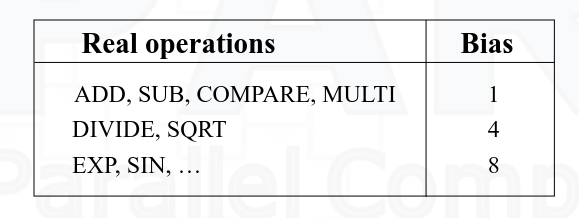
\includegraphics[width=0.7\linewidth]{img/normalized-gflops.png}
	\caption{Esempio di bias per operazioni FP.}
	\label{fig:normalized-gflops}
\end{figure}

Un frammento di codice con operazioni un'operazione ADD, una DIVIDE e una SIN, si calcola avere 12 operazioni FP normalizzate.
\newpage
\begin{exercise}
	Il programma Spice viene eseguito su una DECstation 3100 in 0,094 secondi. Il numero di operazioni in virgola mobile eseguite dal programma è riportato nella tabella.
	\begin{table}[ht]
		\centering
		\scriptsize
		\begin{tabular}{|l|r|}
			\hline
			addD & 25,999,440
			\\\hline
			subD & 18,266,439
			\\\hline
			mulD & 33,880,810
			\\\hline
			divD & 15,682,333
			\\\hline
			compareD & 9,745,930
			\\\hline
			negD & 2,617,846
			\\\hline
			absD & 2,195,930
			\\\hline
			convertD & 1,581,450
			\\\hline
			\textbf{totale} & \textbf{109,970,178}
			\\\hline
		\end{tabular}
	\end{table}
	Calcolare:
	\begin{itemize}
		\item I GFLOPS del programma.
		\item I GFLOPS normalizzati.
	\end{itemize}
\end{exercise}
\begin{solution}
	\begin{align*}
		\textsc{ci\textsubscript{ott}} &= \textsc{ci\textsubscript{non ott}}\cdot \left[(1-0.3)\cdot \left(1-\frac{1}{3}\right)\right]=0.9 \cdot \textsc{ci\textsubscript{non ott}}\\
		\textsc{ci\textsubscript{ott}} &= \textsc{cpi\textsubscript{non ott}}=1\\
		\textsc{t\textsubscript{\textsc{clock\textsubscript{ott}}}} &= 1.05 \cdot \textsc{t\textsubscript{\textsc{clock\textsubscript{non ott}}}}\\
		\textsc{t\textsubscript{cpu\textsubscript{ott}}} &= 0.9 \cdot \textsc{ci\textsubscript{non ott}} \cdot \textsc{cpi\textsubscript{\textsc{non ott}}}\cdot\textsc{t\textsubscript{clock\textsubscript{non ott}}}\\
		&=0.945 \cdot \textsc{ci\textsubscript{non ott}}\cdot \textsc{cpi\textsubscript{non ott}}\cdot \textsc{t\textsubscript{clock\textsubscript{non ott}}}\\
		&= 0.945 \cdot \textsc{t\textsubscript{cpu\textsubscript{non ott}}}
	\end{align*}
\end{solution}















    \section{Prospettive sulla programmazione parallela}
Uno degli aspetti più importante è analizzare il problema e capire se può essere parallelizzato. La parallelizzazione del codice parta a dei miglioramenti delle performance solo se il workload (peso computazionale) è non indifferente.


Partiamo con un po' di definizioni:
\begin{itemize}
    \item Task: arbitrario pezzo di lavoro/sequenza di codice in una computazione parallela. Viene eseguito sequenzialmente, la concorrenza si ha solo tra le task;
    una task è una sequenza di istruzioni che andiamo a identificare, è una parte del programma.
    \item Processo/thread: entità astratta che performa le task assegnate ai progetti. I processi comunicano e si sincronizzano per eseguire le lo task.
    \item Processore: motore fisico sul quale si eseguono i processi. Più thread possono essere eseguiti sullo stesso processore, un thread non può essere eseguita su più processori.
\end{itemize}

\subsection{Step per creare un programma parallelo}
Possiamo identificare 4 passi nella creazione di un programma parallelo:
\begin{enumerate}
    \item Decomposizione della computazione in task -> parto dall'algoritmo risolutivo e identifico tutte le task che lo compongono (divido il problema in sottoproblemi);
    \item Assegnamento delle task ai processi (mappiamo le task identificate nelle thread disponibili); 
    \item Orchestrazione degli accessi ai dati, della comunicazione e della sincronizzazione -> si capisce come raggruppare i processi in unità da eseguire in parallelo;
    \item Mapping dei processi ai processori. Ovviamente, un processo non può essere assegnato a più unità di calcolo.
\end{enumerate}

Le fasi di \textbf{decomposizione} e \textbf{assegnamento} compongono la fase di partizionamento del problema (partiamo da un problema grosso e lo dividiamo su processi computazionale). Qui in pratica è dove identifichiamo il livello di parallelismo.

\subsubsection{Comprensione del problema/programma}
Il primo reale step da eseguire resta però il capire il problema e/o il programma. Se stiamo partendo da un programma sequenziale già scritto, dobbiamo per forza capire come funziona per poterlo parallelizzare, mentre nel caso del problema dobbiamo capire se questo è anche parallelizzabile. 
In generale quello che dobbiamo fare è:
\begin{enumerate}
    \item Identificare gli hotspot del programma: rappresentano le parti più "pesanti" del codice e sono solitamente identificati dopo aver fatto profiling\footnote{I tool di profiling eseguono il codice e, assieme al suo risultato, ritornano anche un report che può contenere: il numero di invocazioni a funzione per ogni funzione del codice, il tempo impiegato da ogni esecuzione di ogni funzione, quali parti del codice sono più usate, ...} e analisi delle performance (tramite appositi tool). Gli hotspot sono generalmente le sezioni in cui si concentra la parallelizzazione.
    \item Identificare i bottleneck del programma: rappresentano i punti del codice che sono più lente ad eseguire (come ad esempio le sezioni dedicate all'I/O). Una possibile strada che si può seguire per i bottleneck consiste nel trasferire la loro esecuzione sulla GPU, in modo da non dover rallentare la CPU. Possiamo quindi vedere due livelli di parallelismo: il primo dato dalla GPU che parallelizza la funzione, mentre il secondo dato dalla concorrenza di esecuzione di CPU e GPU.
    \item Identificare gli inibitori al parallelismo: analizzare il problema significa anche identificare gli inibitori del parallelismo, che sono quei fattori che impediscono di parallelizzare il codice. Generalmente, un inibitori dal parallelismo è la dipendenza delle task, dove il risultato di quella successiva dipende dal risultato di quella precedente.
\end{enumerate}

\underline{Esempio di problema parallelizzabile}: Calcolare l'energia potenziale per ciascuna delle diverse migliaia indipendenti Conformazioni di una molecola. Al termine, trova la conformazione energetica minima. Ogni conformazione molecolare è indipendentemente determinabile e il calcolo della conformazione energetica minima è parallelizzabile.
\\

\underline{Esempio di problema non-parallelizzabile}: Calcolare la serie di Fibonacci. Questo problema non è parallelizzabile in quanto il calcolo attuale dipende dai calcoli precedenti (il termine $k+2$ è dato dalla somma dei termini $k+1$ e $k$). 
\\



\subsubsection{Decomposizione}
Nella scomposizione andiamo ad identificare task sufficiente affinché ce ne sia abbastanza da poter tenere le thread, e i corrispondenti processori, sempre occupati. Questo significa che se abbiamo una macchina con 100 processori, che possono andare tutti in parallelo, dobbiamo avere un pool di task sufficientemente grande da poter tenere occupati tutti i processori anche nel momento in cui una delle task si blocca. Infatti capiterà che una task arrivi al punto in cui necessità di dati da un'altra task o di eseguire operazioni di I/O, restando quindi bloccata e lasciando inutilizzato il processore. Quello che vogliamo evitare è appunto il suo utilizzo, che possiamo evitare se disponiamo di un'altra task pronta ad essere eseguita appena un processore si libera. Dei core/processori lasciati in stallo (inutilizzati) ci ritroviamo con uno spreco di risorse.
Per farla semplice, ci serve un numero di task sufficiente a permetterci di rimpiazzare immediatamente quelle "bloccate" per evitare l'inutilizzo dei processori.

Esistono due modi per scomporre in task:
\begin{itemize}
    \item Scomposizione di dominio: prevede di scomporre i dati del problema, facendo lavorare poi ogni task su una porzione dei dati. Esistono vari modi di partizionare i dati, la soluzione migliore generalmente dipende dal modo in cui sono memorizzati i dati sul pc.

    I problemi, che siano monodimensionale che bidimensionali, possono essere scomposti, ad esempio, in blocchi o cicli (figure \ref{fig:domain-decomposition}). Un fattore importante da tenere presente è il bilanciamento del carico. se siamo sicuri che il tempo impiegato dalla prima thread sul blocco A corrisponde a quello impiegato dalla seconda thread sul blocco B e così via per il resto dei blocchi, allora abbiamo un carico bilanciato. Questo di solito è il caso per problemi lineari. Quando però abbiamo problemi più complessi, il carico di lavoro di una thread diventa imprevedibile. In questo caso potrebbe essere più ottimale aumentare i blocchi facendo in modo che il primo processore che si libera vada a prendere la successiva thread in attesa.
    \begin{figure}[th]
    	\centering
    	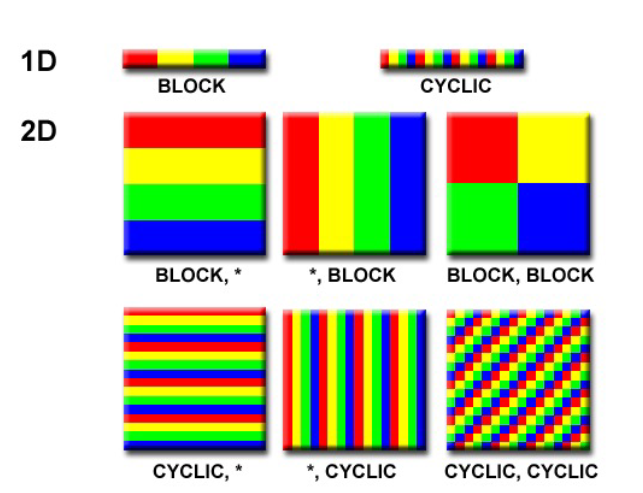
\includegraphics[width=0.7\linewidth]{img/domain-decomposition.png}
    	\caption{Esempio di decomposizione del dominio.}
    	\label{fig:domain-decomposition}
    \end{figure}

    \item Scomposizione funzionale: ci si concentra sull'elaborazione che deve essere fatta piuttosto che sui dati manipolati dalla computazione. Il problema è quindi scomposto rispetto al lavoro che deve essere fatto. Ogni task esegue parte del lavoro totale.
\end{itemize}

La scomposizione è compito del programmatore, che può essere supportato da tool automatici (campo di ricerca).

\underline{Esempio di parallelizzazione}
\\

Data un'immagine $NxN$ vogliamo:
\begin{itemize}
    \item Raddoppiare la luminosità di ogni pixel;
    \item Calcolare la media di tutti i pixel.
\end{itemize}

Una risoluzione sequenziale di questo problema costa un tempo totale di $2N^2$, con ogni step che ne costa $N^2$ (figure \ref{fig:esecuzione-sequenziale}). 
\begin{figure}[th]
	\centering
	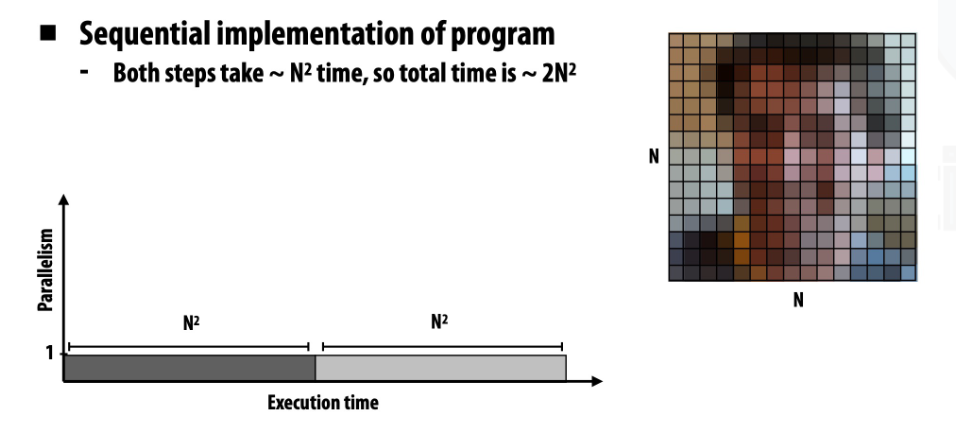
\includegraphics[width=0.7\linewidth]{img/esecuzione-sequenziale.png}
	\caption{Esecuzione sequenziale.}
	\label{fig:esecuzione-sequenziale}
\end{figure}

Una possibile strategia di parallelizzazione potrebbe consiste nell'eseguire in parallelo lo step 1, portando il tempo necessario a completare questa fase a $N^2/P$ (figure \ref{fig:esecuzione-parallela-1}), dove $P$ rappresenta il numero di processori disponibili. Lo speedup ottenuto sarebbe:
\begin{align*}
    speedup &\le \frac{2n^2}{\frac{n^2}{p} + n^2}\\
    &\le 2
\end{align*}

\begin{figure}[th]
	\centering
	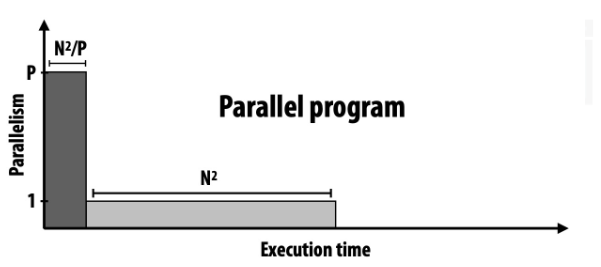
\includegraphics[width=0.7\linewidth]{img/esecuzione-parallela-1.png}
	\caption{Primo tentativo di parallelismo.}
	\label{fig:esecuzione-parallela-1}
\end{figure}

Una strategia più efficiente consiste nel parallelizzare parzialmente anche il secondo step, computando le somme parziali in parallelo (figure \ref{fig:esecuzione-parallela-2}). I tempi diventano:
\begin{align*}
    \text{Tempo step 1 } &= \frac{N^2}{P}\\
    \text{Tempo step 2 } &= \frac{N^2}{P} + P\\
\end{align*}

con speedup:
\begin{align*}
    speedup \le \frac{2n^2}{\frac{n^2}{p} + p}\\
\end{align*}

\begin{figure}[th]
	\centering
	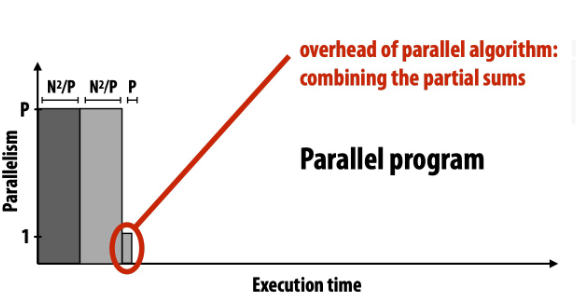
\includegraphics[width=0.7\linewidth]{img/esecuzione-parallela-2.png}
	\caption{Secondo tentativo di parallelismo.}
	\label{fig:esecuzione-parallela-2}
\end{figure}

\subsubsection{Assegnamento}
In questa fase andiamo a specificare il meccanismo con cui dividere le task tra i processi. Per semplicità, possiamo vedere le task come "cose da fare", mentre i processi/thread come i "lavoratori". Abbiamo fatto la scomposizione, sappiamo quanti e quali sono le thread, cerchiamo ora di fare un assegnamento che ci garantisca un certo livello di carico. 
Un approccio strutturato solitamente funziona bene, possiamo seguire euristiche ben conosciute o anche ispezionare attentamente il codice.


Il \textbf{load balancing} (bilanciamento del carico di lavoro) fa riferimento alla pratica di distribuzione delle task tra le thread affinchè tutte le thread siano occupate tutto il tempo. Possiamo anche definirlo come la riduzione al minimo dei tempi di inattività del processo. Questo passo è molto significativo per le perfromance. Ad esempio, se tutti i processi fossero soggetti ad un punto che funge da barriera di sincronizzazione, le performance globali verrebbero determinate dalla task più lenta.
\begin{figure}[th]
	\centering
	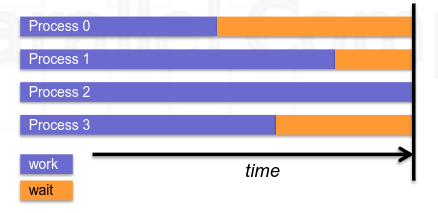
\includegraphics[width=0.7\linewidth]{img/barrier-sync.png}
	\caption{Esempi di punto di sincronizzazione.}
	\label{fig:barrier-sync}
\end{figure}

Possiamo ottenere il load balancing in più modi:
\begin{enumerate}
    \item Dividendo equamente le task tra i processi disponibili:
    \begin{itemize}
        \item In caso di operazioni su array/matrici, dove ogni processo esegue operazioni simili, il dataset viene distribuito in modo uniforme tra i processi;
        \item Per le iterazioni di un ciclo dove il lavoro svolto da ogni loop è similare, le iterazioni vengono distribuite uniformemente tra i processi;
        \item Se si utilizza un mix eterogeneo di macchine con performance variabili, è consigliato utilizzare dei tool di analisi delle performance per individuare carichi sbilanciati e aggiustare di conseguenza.
    \end{itemize}
    \item Usando un assegnamento dinamico del lavoro: alcune classi generano un carico di lavoro sbilanciato anche se i dati sono distribuiti egualmente tra il processi, come:
    \begin{itemize}
        \item Array sparsi;
        \item Adaptive grid methods, dove alcuni processi potrebbero dover perfezionare la propria mesh, mentre altri no;
        \item N-body simulations, dove alcune particelle potrebbero migrare verso/dal dominio del proprio processo di origine verso quello di un altro processo, oppure dove alcune particelle richiedono più lavoro rispetto ad altre.
    \end{itemize}
    Quando l'ammontare di lavoro che ogni thread performerà è variabile (non intenzionalmente ovviamente), è utile usare un approccio \textbf{scheduler – task pool}. In questo modo, appena un processo finisce, si mette in coda per ottenere un nuovo pezzo di lavoro.
    Inoltre, potrebbe diventare necessario disegnare un algoritmo che rileva e gestire sbilanciamento mentre questi si verificano dinamicamente nel codice.
\end{enumerate}

La \textbf{granularità} rappresenta una misura qualitativa del rapporto tra computazione e comunicazione. Generalmente i periodi di computazione sono separati da quelli di comunicazione da eventi di sincronizzazione. Relativamente al parallelismo, la granularità si divide in:
\begin{itemize}
    \item Fine grain parallelism (parallelismo a grana fine): si effettuano relativamente piccole quantità di lavoro computazionale tra gli eventi di comunicazione. Abbiamo quindi un basso rateo tra computazione e comunicazione. Facilita il load balancing; implica un elevato overhead di comunicazione e meno opportunità per il miglioramento delle performance. Se la granularità è troppo fine è possibile che l'overhead richiesto per comunicazione ee sincronizzazione tra le task richieda più tempo della computazione vera e propria.





    \item Coarse grain parallelism (parallelismo a grana grossa): si effettuano relativamente grandi quantità di lavoro computazionale tra gli eventi di comunicazione/sincronizzazione. Abbiamo quindi un alto rateo tra computazione e comunicazione. Implica più opportunità per un incremento delle performance, ma rende più difficile bilanciare il carico di lavoro efficientemente
\end{itemize}














\end{document}